\section{动态规划初步------背包问题}
这一部分,我们将开始对背包问题的研究。

准备好了吗?

限于篇幅以及我的姿势水平,在这一部分里我们仅研究最基础的动态规划问题。本人的目的不是想让你们通过这节课精通DP,而是想让你们对于DP有一个初步的了解,会做基本的DP题,并懂得举一反三,更重要的是\textbf{理解DP的思想}。
\subsection{背包问题是什么?}
\begin{definition}[背包问题(Knapsack problem)]是一种组合优化的NP完全问题。问题可以描述为:给定一组物品,每种物品都有自己的重量和价格,在限定的总重量内,我们如何选择,才能使得物品的总价格最高。
\end{definition}

以上就是百度百科对背包问题的定义,所谓“NP完全问题”是指这个问题具有多项式解法,即时间复杂度可以写成多项式形式$O(n^k\ , n \in\ $\textbf{N}$_+$
且$k$为已知常数$)$。背包问题本质上就是一种最优化组合问题,符合DP的要求,所以DP可以完成对背包问题的求解。时间复杂度是$O(n^2)$,空间复杂度是$O(n^2)$,优化后可以做到$O(n)$。

背包问题可以分为以下8类:
\begin{itemize}
	\item{01背包问题}
	\item{完全背包问题}
	\item{多重背包问题}
	\item{混合背包问题}
	\item{二维背包问题}
	\item{分组背包问题}
	\item{有依赖的背包问题}
	\item{泛化物品}
\end{itemize}

每种问题都有类似的做法,同时也有它们各自的不同之处。下面我们从最基础的01背包开始讲起,它非常重要,是后面所有背包问题的基础,一定要掌握。

\subsection{01背包问题}
\subsubsection{简介}
\begin{definition}[01背包问题]一个背包总容量为$V$,现在有$N$个物品,第$i$个物品体积为$weight[i]$,价值为$value[i]$,现在往背包里面装东西,怎么装能使背包的内物品价值最大?\end{definition}

以上就是\rm{01}背包的定义了。

看到此类问题,我们的第一反应大概就是贪心了。然而贪心是肯定不行的。

为什么不行?举一个例子:
\begin{example}最少硬币找零问题:给予不同面值的硬币若干种(每种硬币个数无限多),用若干种硬币组合为某种面额的钱,使硬币的的个数最少。\end{example}

在现实生活中,我们往往使用的是贪心算法,比如找零时需要13元,我们先找10元,再找2元,再找1元。这是因为现实生活中的硬币(纸币)种类特殊。如果我们的零钱可用的有1、2、5、9、10。我们找零18元时,贪心算法的策略是:10+5+2+1,四种,但是明明可以用两个9元的啊。所以肯定不能用贪心。

那么我们该怎么办?dalao们思考两分钟,不然我们先想一想搜索的方法吧(如果秒掉了的话就看看下面的图)。

\begin{center}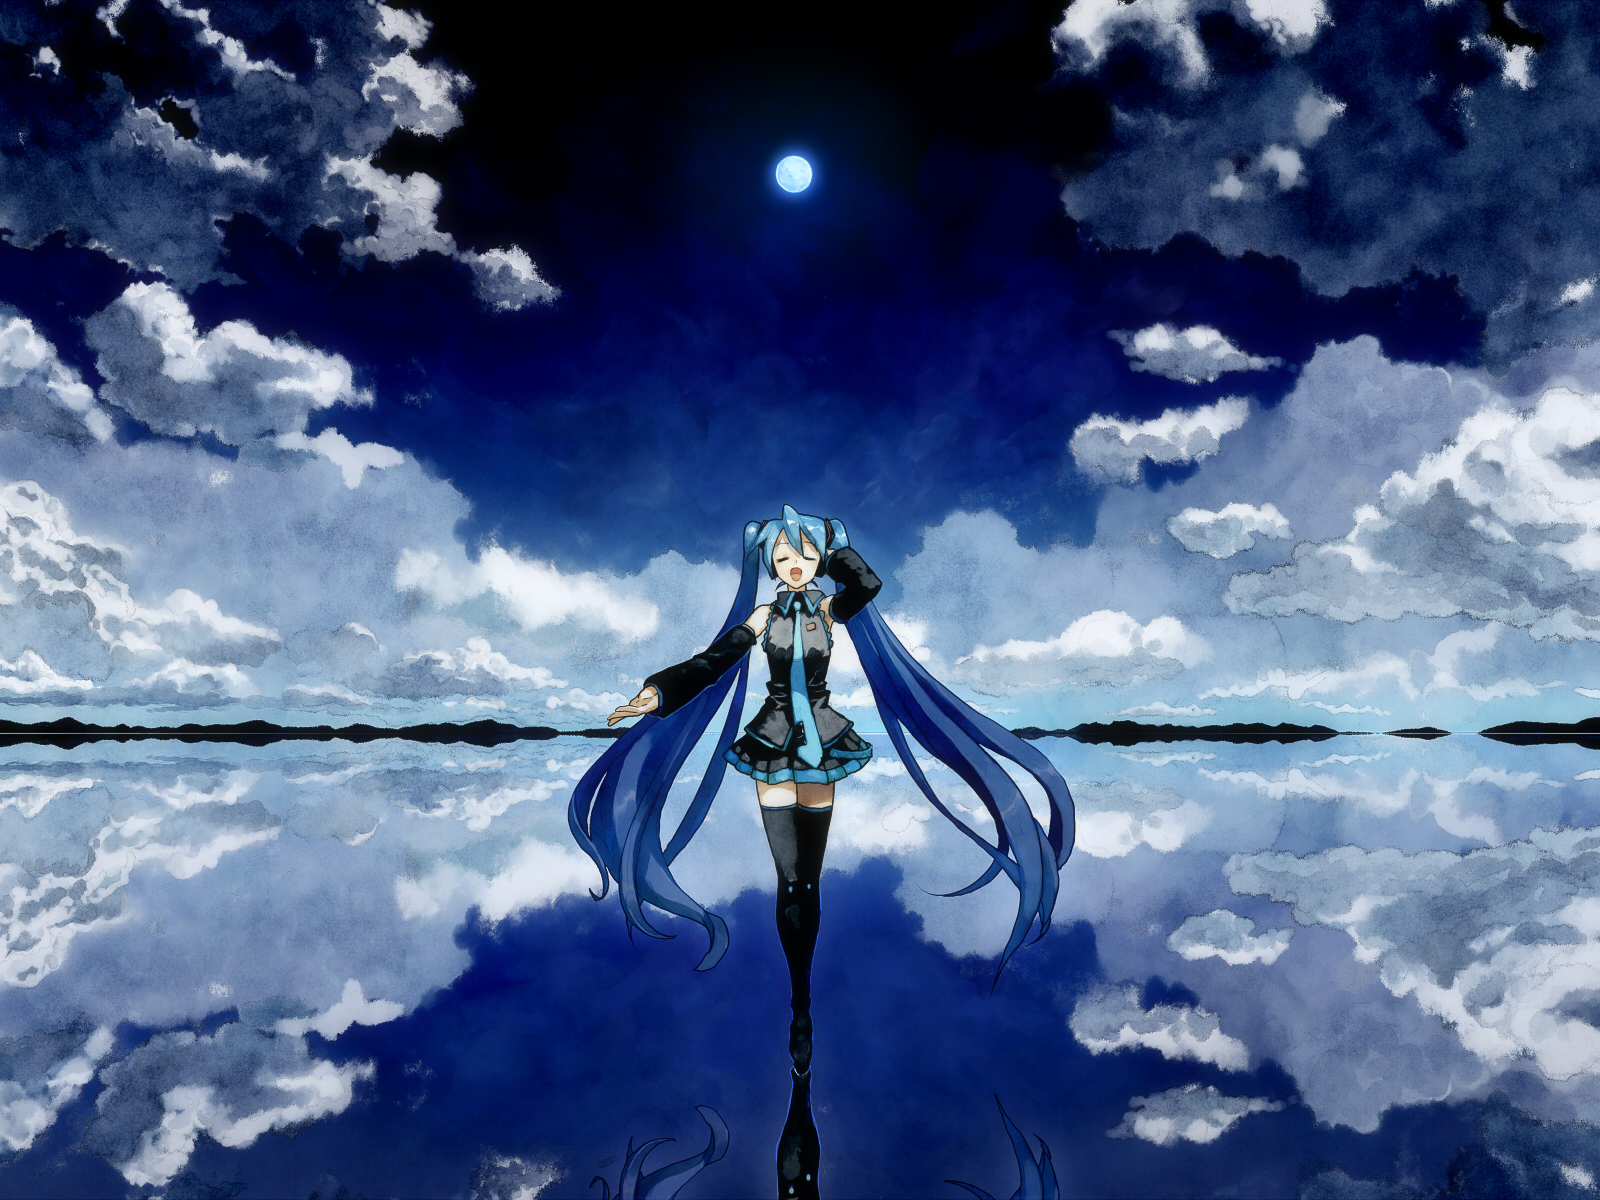
\includegraphics[scale=0.8]{6081163_p0.jpg}\end{center}
\newpage
\begin{example}\rm{01}背包问题:有$n$个重量和价值分别为$w[i]$和$v[i]$的物品。从这些物品中挑出总重量不超过$W$的物品,求所有挑选方案中价值总和的最大值。\end{example}

\subsubsection{搜索}
相信dalao们都能一眼秒掉这个问题。利用搜索,我们可以很快解决这个问题。代码如下:
\begin{enumerate}
\item \begin{minted}{C++}
void dfs(int index,int sumw,int sumv)//index:数组下标,sumw:当前情况的物品体积,sumv:当前情况的物品价值
{ 
    if(index>n)  
    {  
        if(sumw<=T&&sumv>maxvalue)  
            maxvalue=sumv;  
        return;  
    }  
    dfs(index+1,sumw+w[index],sumv+v[index]);//选
    dfs(index+1,sumw,sumv);//不选
}\end{minted}
\item \begin{minted}{C++}  
int W, n;
int w[MAXN], v[MAXN];  
int dfs(int i, int j)
{  
    int res;  
    if(i == n) res = 0;   
    else if(j < w[i]) res = dfs(i+1, j);  
    else res = max(dfs(i+1, j), dfs(i+1, j-w[i])+v[i]);  
    return res;  
}
\end{minted}
\end{enumerate}
然而以上代码有一个问题。时间复杂度太高,$O(2^n)$显然不能满足我们的要求,不能只过$n\leq15$的这部分数据啊。

考虑优化一下。记忆化搜索?
\begin{minted}{C++}
int W, n;    
int w[MAXN], v[MAXN];  
int dp[MAXN][MAXN];  
int dfs(int i, int j)
{  
    if(dp[i][j] >= 0) return dp[i][j];  
    int res;   
    if(i == n) res = 0; 
    else if(j < w[i]) res = dfs(i+1, j);   
    else res = max(dfs(i+1, j), dfs(i+1, j-w[i])+v[i]);  
    return dp[i][j] = res;  
}
\end{minted}

开一个二维数组记录一下每次搜索到的结果,这样时间复杂度就降低到了$O(nW)$,似乎不错。
\subsubsection{二维DP}
不然把上面的那个递归转化一下,转化成递推?简化一下代码?

设状态$dp[i+1][j]$表示从前$i$个物品挑选出总重量超过$j$的物品时,背包中的最大价值,那么根据题意,我们有以下递推式(就是状态转移方程):
\begin{equation*}
	dp[i+1][j]=\begin{cases}
		dp[i][j]                        & ,j<w[i]   \\
		\max\{dp[i+1][j],dp[j-w[i]]+v[i]\} & ,其他情况.
	\end{cases}
\end{equation*}

我来解释一下上面的状态转移方程。首先,要明确状态以及状态之间的转移过程。容易看到,在DFS中状态有两个参数$i,j$,分别代表\underline{当前是第几}\\\underline{个物品}以及\underline{当前背包的剩余容量}。所以DP也应该有两个状态,含义相同。如果背包容量不足了,那么就不取,价值不变;否则有两种决策:
\begin{itemize}
	\item{取当前物品,背包剩余容量减当前物品的体积,当前所获得价值加当前物品的价值;}
	\item{不取当前物品,考虑下一个物品。}
\end{itemize}

在这两种决策中取一个最优解即可。DP同理,只是将决策写成递推式的形式,本质和搜索是相同的。

所以我们得到以下代码:

\begin{minted}{C++}
for(int i = 0; i < N; ++i)
        for(int j = 0; j <= W; ++j)
            if(j < w[i])
                dp[i][j] = dp[i + 1][j];
            else
                dp[i][j] = max(dp[i + 1][j], dp[i + 1][j - w[i]] + v[i]);
\end{minted}
\textbf{重要提示:}\textcolor{red}{在DP中有一点非常重要,那就是\underline{\textbf{对状态数组的初始化}},万万不可忽略!在本题中,如果我们将数组开成全局变量,那么就不需要(\textbf{而不是可以忽略!})对状态数组的初始化,因为初始状态什么都没有放,价值都为0,同时全局变量默认的初始值都是0。\textbf{这只是一个个例!}很多题目都是\textbf{需要}对状态数组进行初始化的。在做DP题时,一定要先对初始状态进行初始化,否则\textbf{你极有可能获得0分,即使你的状态转移方程没有推错!}}
\subsubsection{一维DP}
考虑将前面的二维DP优化一下。

好像时间复杂度已经是最优化了,但是空间复杂度好像还有待提升。

看看刚才的状态转移方程或者代码。转移前后的状态有什么关系?

共同之处在于:$dp[i][j]=dp[i+1][Something]$,通过这个性质,我们可以压去这个方程的第一维,并且不取新的物品与背包没有空间时的情况相同,所以我们可以得到以下状态转移方程:
\begin{equation*}dp[i]=\max\{dp[i],dp[i-w[j]]+v[j]\},\ i\geq w[j]\end{equation*}

时间复杂度:$O(n^2)$,空间复杂度$O(n)$。

这个状态转移方程非常重要,在以后的学习中还会多次用到。

有什么问题随时问我就好,我会很乐意帮忙的。有不会的必须弄明白,因为01背包问题是所有其他背包问题的基础。

\textbf{重要提示:}\textcolor{red}{\textbf{请特别注意此题的枚举顺序,由于$dp[i]$是由$dp[i-w[j]]$转移来的,为了避免后效性需要倒序枚举背包的容量,这也是压维优化DP的特征}}(但不是所有的压维优化DP都需要倒序枚举)。

\note
\section*{\textcolor{white}{?????}}
\begin{quote}
	\textcolor{white}{やがて\ruby{日}{ひ}が\ruby{過}{す}ぎ \ruby{年}{とし}が\ruby{過}{す}ぎ\\
		光阴飞逝 岁月如梭}

	\textcolor{white}{\ruby{古}{ふる}い\ruby{荷物}{にもつ}も ふえて\\
		陈旧的负担 增加了}

	\textcolor{white}{あなたが かわっても\\
		你即使 自己改变}

	\textcolor{white}{\ruby{失}{な}くしたくないものは\\
		也不愿失去的事物}

	\textcolor{white}{ワタシに あずけてね\\
		就交由我 来保管吧}

	\ \\

	\textcolor{white}{\ruby{時}{とき}の\ruby{流}{なが}れも \ruby{傷}{きず}の\ruby{痛}{いた}みも\\
		不论是时间的流逝 受伤的苦痛}

	\textcolor{white}{\ruby{愛}{あい}の\ruby{深}{ふか}さも あなたの\ruby{声}{こえ}も\\
		爱意的深切 还是你的话声}

	\textcolor{white}{ワタシは\ruby{知}{し}らない だけど\ruby{歌}{うた}は\\
		即使我全都一无所知 依然继续地}

	\textcolor{white}{\ruby{歌}{うた}はうたえるわ だからきいて\\
		尽我所能的歌唱 所以请好好倾听吧}

	\textcolor{white}{もしもあなたが \ruby{望}{のぞ}むのなら\\
		若是你如此 期望的话}

	\textcolor{white}{\ruby{何}{なん}\ruby{度}{ど}でも \ruby{何}{なん}\ruby{度}{ど}だって\\
		不论几次 不论多少次}

	\textcolor{white}{かわらないわ あのときのまま\\
		不会改变的 从那时以来不曾变过的}

	\textcolor{white}{ハジメテノオトのまま...\\
		那不变的初次歌声...}

	\begin{flushright}\textcolor{white}{------「ハジメテノオト」}\end{flushright}
\end{quote}

\subsection{完全背包问题、多重背包问题与混合背包问题}
这一节内容看起来会比较多,但是因为有了前面一节的基础,相信大家也能够很容易的掌握。

\begin{definition}[完全背包问题]一个背包总容量为V,现在有N个物品,第i个物品体积为weight[i],价值为value[i],每个物品都有无限多件,现在往背包里面装东西,怎么装能使背包的内物品价值最大?\end{definition}

\begin{definition}[多重背包问题]一个背包总容量为V,现在有N个物品,第i个物品体积为weight[i],价值为value[i],每个物品有num[i]($num[i]\geq 1$)件,现在往背包里面装东西,怎么装能使背包的内物品价值最大?\end{definition}

\begin{definition}[混合背包问题]一个背包总容量为V,现在有N个物品,第i个物品体积为weight[i],价值为value[i],有的物品只有一件,有的物品有num[i]($num[i]\geq 1$)件,有的物品有无限多件,现在往背包里面装东西,怎么装能使背包的内物品价值最大?\end{definition}

以上是对这三种背包问题的定义,希望大家能够理解。可以发现这三种问题非常类似,也有不同。下面我就逐一来讲解。

\subsubsection{完全背包问题}

还记得上一节讲的01背包的一维状态转移方程吗?当时我曾经说过“为了避免后效性需要倒序枚举”,完全背包问题因为每个物品都有无限多件,所以可以利用这个后效性,正序枚举即可。

完全背包问题就讲完了。

\subsubsection{多重背包问题}
对于多重背包问题,我们可以考虑每一件物品都拆成01背包来做,N种物品,分别枚举每种物品的每一件即可。

就是加一层循环,枚举每一种物品中的每一件的状态。代码如下:
\begin{minted}{C++}
for(int i=0;i<N;i++)
    for(int j=0;j<num[i];j++)
        for(int k=V;k>=v[i];k--) 
            dp[k]=max(dp[k],dp[k-v[i]]+w[i]);
\end{minted}

这里稍微加了一点常数优化,注意最内层的循环,没有从V枚举到0,因为背包容量小于物品体积时对答案没有任何贡献(本来就放不下,当然不能硬塞)。

\subsubsection{混合背包问题}
这种问题就是把前面三种背包问题混合起来,所以我们只需要把前面三种背包都写一遍(实际上只要写完全背包和多重背包即可),然后加个判断就行了。

以下代码假设物品数量已经读入,第i个物品的数量用num[i]表示,且当num[i]=-1时,表示这个物品有无限多件:
\begin{minted}{C++}
for(int i=0;i<N;i++)
{
    if(num[i]!=-1)
    {
        for(int j=0;j<num[i];j++)
            for(int k=V;k>=v[i];k--) 
                dp[k]=max(dp[k],dp[k-v[i]]+w[i]);
	}
    else
    {
        for(int j=v[i];j<=V;j++)
            dp[j]=max(dp[j],dp[j-v[i]]+w[i]);
    }
}
\end{minted}

这三种问题是不是很简单呢?有不会的问题可以提问。
\note

\section*{\textcolor{white}{?????}}
\begin{quote}
	\textcolor{white}{\ruby{想}{おも}いよ\ruby{届}{とど}け \ruby{君}{きみ}に\\
		该怎么办才好…! 思念啊请传达给你}

	\ \par

	\textcolor{white}{お\ruby{願}{ねが}い\ruby{時間}{じかん}を\ruby{止}{とめ}めて \ruby{泣}{な}きそうなの\\
		拜托时间请停下来 感觉快要哭出来了}

	\textcolor{white}{でも\ruby{嬉}{うれ}しくて \ruby{死}{し}んでしまうわ!\\
		但是又好高兴 高兴到快要死掉了!}

	\ \par

	\textcolor{white}{メルト \ruby{駅}{えき}に\ruby{着}{つ}いてしまう……\\
		Melt 终究还是抵达了车站……}

	\ \par

	\textcolor{white}{もう\ruby{会}{あ}えない \ruby{近}{ちか}くて \ruby{遠}{とお}いよ だから\\
		再也见不到面了 那么的近 却又是那么的遥远 所以}

	\ \par

	\textcolor{white}{メルト \ruby{手}{て}をつないで\ruby{歩}{ある}きたい!\\
		Melt 想要手牵着手 一起前进!}

	\textcolor{white}{もうバイバイしなくちゃいけないの?\\
		已经是不得不说再见的时候了吗?}

	\ \par

	\textcolor{white}{\ruby{今}{いま}すぐ わたしを\ruby{抱}{だ}きしめて!\\
		现在马上 抱紧我!}

	\ \par

	\textcolor{white}{……なんてね\\
		……只是想想而已}
	\begin{flushright}\textcolor{white}{------メルト}\end{flushright}
\end{quote}
\newpage
\subsection{二维背包问题与分组背包问题}
\subsubsection{二维背包问题}
\begin{definition}[二维背包问题]对于每件物品,具有两种不同的费用;选择这件物品必须同时付出这两种代价;对于每种代价都有一个可付出的最大值(背包容量)。问怎样选择物品可以得到最大的价值。\end{definition}

定义比较长,但是事实上就是背包问题的再次综合。状态加一维表示第二种代价,然后套用适当的背包模板即可。注意最好使用一维的DP进行状态转移,否则可能会爆空间。


设第$i$件物品所需的两种代价分别为$a[i]$和$b[i]$。两种代价可付出的最大值(两种背包容量)分别为$u$和$v$。第$i$件物品的价值为$value[i]$。

三维状态转移方程:$f[i][u][v] = \max(f[i-1][u][v] , value[i] + f[i-1][u-a[i]][v-b[i]])$

二维状态转移方程(注意需要倒序枚举):$f[i][j] = \max(f[i][j] , value[k]$ $+ f[u-a[k]][v-b[k]])$

时间复杂度:$O(n^3)$,空间复杂度$O(n^2)$。

\subsubsection{分组背包问题}
\begin{definition}[分组背包问题]有N件物品和一个容量为V的背包。第i件物品的费用是w[i],价值是v[i]。这些物品被划分为k组,每组中的物品互相冲突,最多选一件。求解将哪些物品装入背包可使这些物品的费用总和不超过背包容量,且价值总和最大。\end{definition}

这种问题看起来与前面的问题不同。但实质是相同的。只不过枚举的对象由每一个物品变成每一类物品,然后对每一类物品分别枚举其中的每一个物品即可。

设枚举对象x为第1~k类物品,i为第x类物品中的第i件物品:

状态转移方程:$f[i]=\max\{f[i],f[i-w[i]]+v[i]\},i\in k_x.$
有问题随时问。
\note
\section*{\textcolor{white}{?????}}
\begin{quote}
	\textcolor{white}{\ruby{悲}{かな}しみの\ruby{海}{うみ}に\ruby{沈}{しず}んだ\ruby{私}{わたし} \ruby{目}{め}を\ruby{開}{あ}けるのも\ruby{億劫}{おっくう}\\
		沉入悲伤之海的我 就连想睁开眼也彷佛永劫}

	\textcolor{white}{このままどこまでも\ruby{堕}{お}ちて\ruby{行}{ゆ}き \ruby{誰}{だれ}にも\ruby{見}{み}つけられないのかな\\
		会就此沉沦下去 没人能够找到吗?}

	\ \par

	\textcolor{white}{どこへ\ruby{向}{む}かい、\ruby{何}{なに}をすれば? ふと\ruby{射}{さ}し\ruby{込}{こ}む\ruby{一筋}{ひとすじ}の\ruby{光}{ひかり}\\
		该朝向哪里,何去何从? 突然洒下的一丝光芒}

	\textcolor{white}{\ruby{手}{て}を\ruby{伸}{の}ばせば\ruby{届}{とど}きそうだけど \ruby{波}{なみ}に\ruby{拐}{さら}われて\ruby{見}{み}{失}{うしな}った\\
		虽然好像只要伸出手就能触及 却被海浪卷走失去踪影}

	\ \par

	\textcolor{white}{あれは\ruby{一体}{いったい}なんだったのかな あたたかくて\ruby{眩}{まぶ}しかったの\\
		那究竟是什么呢 既温暖又炫目}

	\textcolor{white}{\ruby{無}{む}{意}{い}{識}{しき}のカウンターイルミネーション\\
		无意识的对抗照明\\
		\ruby{嘘}{うそ}つきは\ruby{誰}{わだれ}?\\
		说谎的到底是谁?}

	\ \par

	\textcolor{white}{\ruby{深海}{しんかい}\ruby{少}{しょう}\ruby{女}{じょ} まだまだ\ruby{沈}{しず}む\\
		深海少女 仍在继续下沉}

	\textcolor{white}{\ruby{暗闇}{くらやみ}の{彼方}{かなた}へ\ruby{閉}{と}じこもる\\
	封闭在黑暗的彼端}

	\textcolor{white}{\ruby{深海}{しんかい}\ruby{少}{しょう}\ruby{女}{じょ} だけど\ruby{知}{し}りたい\\
		深海少女 但想要知道}

	\textcolor{white}{\ruby{心惹}{こころひ}かれるあの\ruby{人}{ひと}を\ruby{見}{み}つけたから\\
		只因找到了那令她倾心的人}
	\begin{flushright}\textcolor{white}{------深海少女}\end{flushright}
\end{quote}
\newpage
\subsection{有依赖的背包问题与泛化物品(选学)}
以下内容为选学,掌握与否都不很重要。讲解以经典例题为主\sout{,不能光\\讲基础的东西不讲题啊}。
\subsubsection{有依赖的背包问题}
\begin{example}金明的预算方案\\
	\textbf{题目描述}

	金明今天很开心,家里购置的新房就要领钥匙了,新房里有一间金明自己专用的很宽敞的房间。更让他高兴的是,妈妈昨天对他说:“你的房间需要购买哪些物品,怎么布置,你说了算,只要不超过N元钱就行”。今天一早,金明就开始做预算了,他把想买的物品分为两类:主件与附件,附件是从属于某个主件的,下表就是一些主件与附件的例子:
	\begin{center}
		\begin{tabular}{|c|c|}
			\hline
			主件   & 附件           \\
			\hline
			电脑   & 打印机、扫描仪 \\
			\hline
			书柜   & 图书           \\
			\hline
			书桌   & 台灯、文具     \\
			\hline
			工作椅 & 无             \\
			\hline
		\end{tabular}
	\end{center}

	如果要买归类为附件的物品,必须先买该附件所属的主件。每个主件可以有0个、1个或2个附件。附件不再有从属于自己的附件。金明想买的东西很多,肯定会超过妈妈限定的N元。于是,他把每件物品规定了一个重要度,分为5等:用整数1~5表示,第5等最重要。他还从因特网上查到了每件物品的价格(都是10元的整数倍)。他希望在不超过N元(可以等于N元)的前提下,使每件物品的价格与重要度的乘积的总和最大。

	设第j件物品的价格为v[j],重要度为w[j],共选中了k件物品,编号依次为$j_1,j_2,j_k$,则所求的总和为:
	\begin{equation*}
		v[j_1]\times w[j_1]+v[j_2]\times w[j_2]+ \cdots +v[j_k]\times w[j_k]
	\end{equation*}

	请你帮助金明设计一个满足要求的购物单。\\
	\textbf{输入输出格式}\\
	\textbf{输入格式}

	输入的第1行,为两个正整数,用一个空格隔开:

	N m (其中N($N<32000$)表示总钱数,m($m<60$)为希望购买物品的个数。)

	从第2行到第m+1行,第j行给出了编号为j-1的物品的基本数据,每行有3个非负整数

	v p q (其中v表示该物品的价格($v<10000$),p表示该物品的重要度(1~5),q表示该物品是主件还是附件。如果q=0,表示该物品为主件,如果q>0,表示该物品为附件,q是所属主件的编号)\\
	\textbf{输出格式}

	输出只有一个正整数,为不超过总钱数的物品的价格与重要度乘积的总和的最大值(不超过200000)。
	\par
	\ \\
	\textbf{输入输出样例}\\
	\textbf{输入样例}
	\begin{minted}{text}
1000 5
800 2 0
400 5 1
300 5 1
400 3 0
500 2 0
\end{minted}
	\textbf{输出样例}
	\begin{minted}{text}
2200
\end{minted}
\end{example}

这道例题是NOIp2006的提高组第二题。结合之前的讲解,dalao们有思路吗?先思考2分钟。

其实很简单,考虑状态:
\begin{itemize}
	\item{主件和两个附件都不选}
	\item{只选择主件,不选择任何一个附件}
	\item{选择主件并选择附件1}
	\item{选择主件并选择附件2}
	\item{选择主件和两个附件}
\end{itemize}

共计5个状态,所以大概需要写5个状态转移方程。

思路和正常向的01背包一致。

设每一件物品的属性:
\begin{itemize}
	\item{m:主件体积}
	\item{a:附件1体积}
	\item{b:附件2体积}
	\item{x:主件价值}
	\item{y:附件1价值}
	\item{z:附件2价值}
\end{itemize}
则我们可以得到:
\begin{eqnarray*}
	f[j]&=&\max(f[j],f[j-m[i]]+x[i])\\
	f[j]&=&\max(f[j],f[j-m[i]-a[i]]+x[i]+y[i])\\
	f[j]&=&\max(f[j],f[j-m[i]-b[i]]+x[i]+z[i])\\
	f[j]&=&\max(f[j],f[j-m[i]-a[i]-b[i]]+x[i]+y[i]+z[i])
\end{eqnarray*}

唯一需要注意的是边界条件(不能出现访问越界的错误)。

\subsubsection{泛化物品}
\begin{example}最佳课题选择\ \\
	\textbf{描述}

	Matrix67要在下个月交给老师n篇论文,论文的内容可以从m个课题中选择。由于课题数有限,Matrix67不得不重复选择一些课题。完成不同课题的论文所花的时间不同。具体地说,对于某个课题i,若Matrix67计划一共写x篇论文,则完成该课题的论文总共需要花费$A_i*x^{B_i}$个单位时间(系数$A_i$和指数$B_i$均为正整数)。给定与每一个课题相对应的$A_i$和$B_i$的值,请帮助Matrix67计算出如何选择论文的课题使得他可以花费最少的时间完成这n篇论文。\ \\
	\textbf{格式}\\
	\textbf{输入格式}

	第一行有两个用空格隔开的正整数n和m,分别代表需要完成的论文数和可供选择的课题数。

	以下m行每行有两个用空格隔开的正整数。其中,第i行的两个数分别代表与第i个课题相对应的时间系数Ai和指数Bi。\\
	\textbf{输出格式}

	输出完成n篇论文所需要耗费的最少时间。
	\ \\
	\textbf{样例}\\
	\textbf{样例输入}
	\begin{minted}{text}
10 3
2 1
1 2
2 1
\end{minted}
	\textbf{样例输出}
	\begin{minted}{text}
19
\end{minted}
	\textbf{数据范围}

	对于$30\%$的数据,$n\leq10, m\leq5$;

	对于$100\%$的数据,$n\leq200, m\leq20, A_i\leq100, B_i\leq5$。
\end{example}

这题非常经典,是泛化物品问题的一道好题。

首先给出泛化物品的定义:
\begin{definition}[泛化物品]在背包容量为V的背包问题中,泛化物品是一个定义域为$[0,V]$中的整数的函数h,当分配给它的费用为v时,能得到的价值就是h(v)。求能获得的最大价值。
\end{definition}

这题实际上不是很难,因为每件物品的数量都只能取整数,即函数$h(x)$的定义域为$x \in\ $\textbf{N}$_+$。所以我们只需要先预处理出$h(x)$在适当范围内的取值,然后套用适当的背包模板即可。

注意状态转移方程中加的部分是预处理出来的数组中对应的函数值。

\note
\section*{\textcolor{white}{?????}}
\begin{quote}
	\textcolor{white}{\ruby{何}{なに}も\ruby{伝}{つた}えないまま\\
		分毫的心意都没传达出}

	\textcolor{white}{さよならは\ruby{言}{い}えないよ\\
		这样子的我说不出再见}

	\ \par

	\textcolor{white}{この\ruby{声}{こえ} \ruby{枯}{か}れても\\
		即使这份 歌声凋零}

	\textcolor{white}{\ruby{消}{き}えない メロディー\\
		旋律依然 不会消失}

	\ \par

	\textcolor{white}{Last Night, Good Night\\
		Last Night, Good Night}

	\textcolor{white}{Last Night, Good Night\\
		Last Night, Good Night}

	\ \par

	\textcolor{white}{いつかは むかえる\\
		等待着那 随时可能}

	\textcolor{white}{\ruby{最後}{さいご}を \ruby{想}{おも}うよ\\
		会来临的 最后一刻}

	\textcolor{white}{\ruby{夜空}{よそら}に \ruby{願}{ねが}うの\\
		向着夜空 寄予心愿}

	\textcolor{white}{ときわの \ruby{笑顔}{えがお}を\\
		愿你永保 那份笑容}

	\textcolor{white}{おやすみ\\
		祝你好梦}
	\begin{flushright}\textcolor{white}{------}\em{\textcolor{white}{``Last Night, Good Night"}}\end{flushright}
\end{quote}

\newpage